\documentclass{article}
\usepackage[left=2.5cm, right=2.5cm, top=2.5cm]{geometry}
\usepackage{indentfirst}
\usepackage{amsmath}
\usepackage{cite}
\usepackage{caption}
\usepackage{subcaption}
\usepackage{graphicx}
\usepackage{float}
\usepackage{amsmath}
\usepackage{listings}
\usepackage{xcolor}
\usepackage{lscape}
\usepackage{pdflscape}
\graphicspath{{./images}}

\lstset { %
	language=C++,
	%backgroundcolor=\color{black!5},
	basicstyle=\footnotesize,
	breaklines=true,
	postbreak=\mbox{\textcolor{red}{$\hookrightarrow$}\space},
	frame=single,
}

%opening
\title{Brown University \\
	Center for Computation and Visualization \\
	HPC Technical Assignment}
\author{Joseph R. Cooke III}

\begin{document}

\maketitle

\newpage

\section{Introduction}
A C++ application to calculate the ordinary least square estimates using the Armadillo library was developed and benchmarked for performance. The following report outlines the benchmarking procedure used along with the code that corresponding to the timing points in the program. 

The outline to the problem was to assume
\begin{equation}
	y = X\beta
\end{equation}
with the estimates to be calculated as
\begin{equation}
	\hat{\beta} = (X^{T}X)^{-1}X^{T}y.
\end{equation}

The completed application is used from the command line with the following syntex:
\begin{lstlisting}
				estOLS -x XMAT -y yVEC -o Output
\end{lstlisting}
where estOLS is the program name, XMAT is a text file containing the matrix $X$ in a space or tab delimited form without a header, yVEC is a text file holding the vector $y$ without a header, and $Output$ is the file name for the calculated estimates output $\hat{\beta}$.

The required dependencies for the Armadillo package are g++, CMake, OpenBLAS, LAPACK, ARPACK and SuperLU. The dependencies can be installed using apt-get with the following command:

\begin{lstlisting}
	sudo apt-get install g++, cmake,  libopenblas-dev, liblapack-dev, libarpack2-dev, libsuperlu-dev
\end{lstlisting}

and the Armadillo package can be installed through apt-get with the following command:

\begin{lstlisting}
	sudo apt-get install libarmadillo-dev
\end{lstlisting}

\section{Benchmark}
The benchmarking for the application was completed using pregenerated random value matrices, XMAT, and vector, yVEC, saved into .txt format. 

Timing was completed using the chrono class in C++ with the following timing metrics to understand where in the program the time was spent. The total elapse time for the program is defined as a measure from the first line of main() to when the timing is displayed in the terminal window which is the last call before the program ends. The XMAT read in time is measured from the opening of the XMAT text file to when the XMAT text file is closed which encapsulates the procedure outlined in Figure \ref{fig:ReadXMAT}. The yVEC read in time is measured from the opening of the yVEC text file to when it closes the yVEC text file which is outlined if Figure \ref{fig:ReadyVEC}. The calculation of the ordinary least squares estimates is measured from declaring the matrices and vectors required to perform the calculation to when it returns the estimates as outlined in Figure \ref{fig:CalculateBeta}. The data writing time is measured from the opening of the text file to it closing the output data file as outlined in Figure \ref{fig:DataWrite}. The individual functions are timed to know the most costly features of the program for future optimization purposes and to determine cost effectiveness of the program. The test system was an Intel Core i7-8550 CPU with 8 GB of system memory.

Table \ref{tab:ET} displays the total elapse times for the program to run under the tested matrices. As observed in Table \ref{tab:ET}, as the $dim \ m$ increases in size, the more time the application takes to run. To further understand the time spent in the program, Table \ref{tab:ETBreakdown} display the individual timing for each of the components of the program. 

\begin{table}[H]
	\centering
	\begin{tabular}{ |c||c|} 
		\hline
		\textbf{XMAT} & \textbf{Total Elapse Time} \\ 
		(dim n x dim m) & (milliseconds)\\
		\hline
		\hline
		(20000,500) & 3088 \\ 
		\hline
		(20000,1000) & 6434 \\ 
		\hline
		(20000,2000) & 15412 \\ 
		\hline
		(20000,10000) & 170041 \\ 
		\hline
	\end{tabular}
	\caption{Total elapse time for estOLS program ran on the test system for the prescribed matrix sizes.} \label{tab:ET}
\end{table}

As observed in Table \ref{tab:ETBreakdown}, the read in of the yVEC text file doesn't vary in all by the last test because its size doesn't vary. The variance in the last test is not significant to investigate. It is also observed that the writing of the estimates to the text file doesn't account for the majority of the time in the application. The two most costly pieces of code is the reading in of the XMAT file and the calculation of the estimates. The reading in of the XMAT file for the first three tested sizes costs the largest amount of computational resources as expected due to the number of points being read and stored to memory. Similarly, as the size of the X matrix increases, the calculation of the estimates also increases and dramatically increases in the final test size. 

Optimization and further work would be most beneficial in the reading in the of XMAT file and the calculation of the estimates.

The data sets in Tables \ref{tab:ET} and \ref{tab:ETBreakdown} were also plotted in Figure \ref{fig:Timing} for visual clarity. 

\begin{table}[H]
	\centering
	\begin{tabular}{ |c||c|c|c|c|} 
		\hline
		\textbf{XMAT} & \textbf{XMAT Read In} & \textbf{yVEC Read In} & \textbf{Estimator Calculation} & \textbf{Data Write} \\ 
		(dim n x dim m) & (milliseconds) & (milliseconds) & (milliseconds) & (milliseconds)\\
		\hline
		\hline
		(20000,500) & 2687  & 6 & 330  & 7 \\ 
		\hline		
		(20000,1000) & 5426  & 6 & 876 & 15 \\ 
		\hline		
		(20000,2000) & 12338  & 6 & 2845 & 21 \\ 
		\hline
		(20000,10000) & 66092  & 7 & 102458 & 283 \\ 
		\hline
	\end{tabular}
	\caption{Individual timing segments for each part of the estOLS program ran on the test system for the prescribed matrix sizes.} \label{tab:ETBreakdown}
\end{table}

\begin{figure}[H]
	\centering
	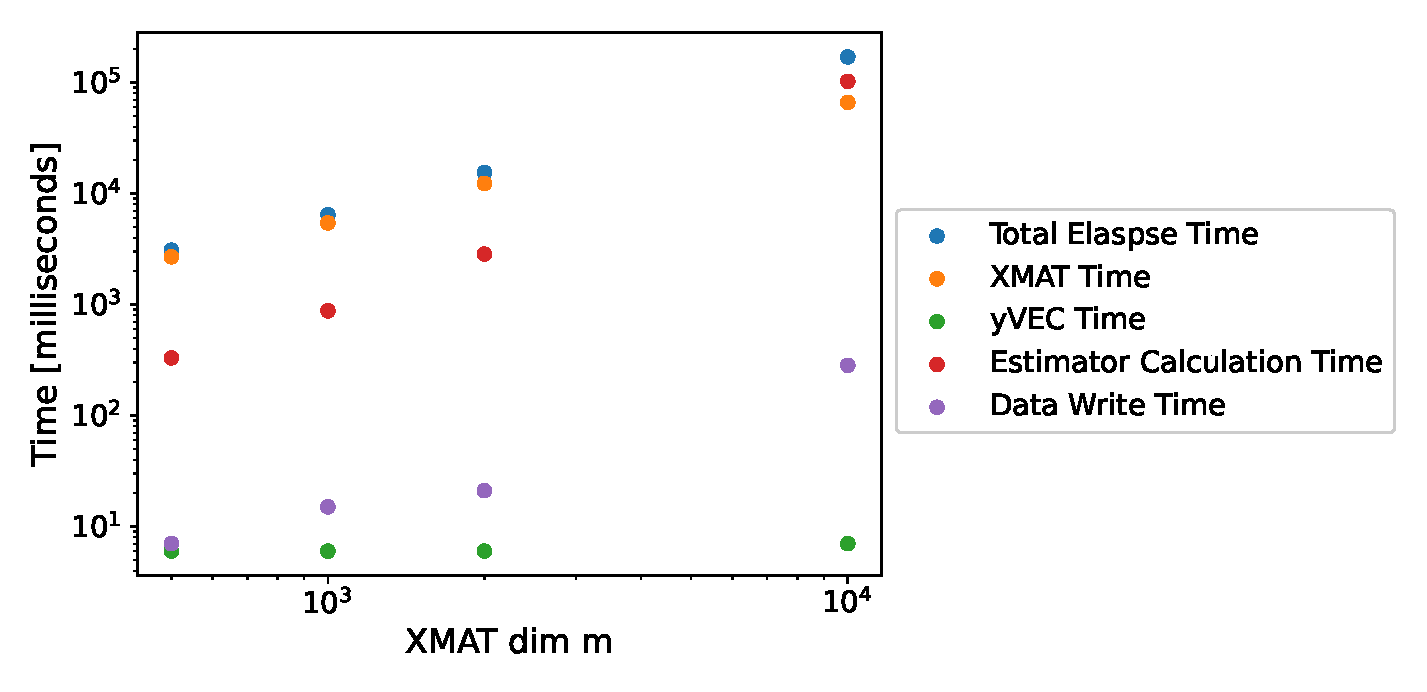
\includegraphics[scale=0.65]{Timing.eps}
	\caption{Timing data from Tables \ref{tab:ET} and \ref{tab:ETBreakdown} from runs on test system. \label{fig:Timing}}
\end{figure}

\section{Code}
The following section contain the functions that are called within main() of the program estOLS. These code blocks are here for reference to the benchmarking of the individual components discussed in the aformentioned section.

\begin{figure}[H]
\begin{lstlisting}
	mat ReadXMAT(string xMAT_input){
		// Opening XMAT text file
		ifstream inputX;
		inputX.open(xMAT_input,ios::in);
		
		// Declaring storage matrix
		mat X;
		
		// Storing data from text file to storage matrix
		X.load(inputX, raw_ascii);
		
		// Closing input file
		inputX.close();
		
		// Returning filled matrix
		return X;
	}
\end{lstlisting}
\caption{ReadXMAT function}\label{fig:ReadXMAT}
\end{figure}

\begin{figure}[H]
\begin{lstlisting}
	vec ReadyVEC(string yVEC_input){
		// Opening yVEC text file
		ifstream inputY;
		inputY.open(yVEC_input,ios::in);
		
		// Declaring storage vector
		vec Y;
		
		// Storing data from text file to storage vector
		Y.load(inputY, raw_ascii);
		
		// Closing input file
		inputY.close();
		
		// Returning filled vector
		return Y;
	}
\end{lstlisting}
\caption{ReadyVEC function}\label{fig:ReadyVEC}
\end{figure}

\begin{figure}[H]
\begin{lstlisting}
	vec CalculateBeta(mat X, vec Y){
		// Declaration of matrix and vector variables
		mat XT, XTX;
		vec Beta;
		
		// Taking the transpose of the input matrix X
		XT = X.t();
		
		// Completing the matrix multiplication
		XTX = XT*X;
		
		// Calculating Beta
		Beta = (inv(XTX))*XT*Y;
		
		// Returning Beta
		return Beta;
	}
\end{lstlisting}
\caption{CalculateBeta function}\label{fig:CalculateBeta}
\end{figure}

\begin{figure}[H]
\begin{lstlisting}
	void DataWrite(string output_name, vec Beta){
		// Opening output file
		ofstream outputData;
		outputData.open(output_name,ios::out);
		
		// Need to specify arma because size() exists in both namespaces
		// Setting bounds for for loop to save data
		int m = arma::size(Beta)[0];
		
		// Writing to output file
		for(int i = 0; i < m; i++){
			outputData << Beta[i] << endl;
		}
		
		// Closing output file
		outputData.close();
	}
\end{lstlisting}
\caption{DataWrite function}\label{fig:DataWrite}
\end{figure}

\end{document}
